\documentclass[a4paper,12pt,oneside]{book}
\usepackage[toc,page]{appendix}
\usepackage{lmodern}
\usepackage[T1]{fontenc}
\usepackage[procnames]{listings}
\usepackage{color}
\usepackage{graphicx}
\usepackage{subfig}
\usepackage{hyperref}
\usepackage{mathtools}
\begin{document}
\definecolor{keywords}{RGB}{255,0,90}
\definecolor{comments}{RGB}{0,0,113}
\definecolor{red}{RGB}{160,0,0}
\definecolor{green}{RGB}{0,150,0}
\lstset{language=Python, 
        basicstyle=\ttfamily\small, 
        keywordstyle=\color{keywords},
        commentstyle=\color{comments},
        stringstyle=\color{red},
        showstringspaces=false,
        identifierstyle=\color{green},
        procnamekeys={def,class}}

\begin{titlepage}
\def \mymaintitle {MatockFS}
\def \mysubtitle {Minimizing disk-cache misses in an asynchronous message-based forensic framework on the Linux platform.}
\def \myauthor {Rob J Meijer}
\def \mysupervisor {Dr Pavel Gladishev} 
\def \mytitle {M.Sc.}
\def \myfield {Forensic Computing and Cyber Crime Investigations}
\def \myschool {School of Computer Science and Informatics}
\def \myuniversity {University College Dublin}

\newcommand{\HRule}{\rule{\linewidth}{0.5mm}}
\center
\HRule \\[0.4cm]
{ \Large \bfseries \mymaintitle}\\[0.4cm]
\emph{\large{\mysubtitle}}
\\[20pt]
{ \large \bfseries \myauthor}\\[0.3cm]
\HRule \\[1.5cm]
A minor thesis submitted in part fulfilment of the degree of \mytitle in \myfield  under the supervision of Dr. \mysupervisor.
\\[10cm]
{\large \myschool}\\[12pt]
{\large \myuniversity}\\[12pt]
{\large \today}
\vfill
\end{titlepage}
%\chapter*{\centering \begin{normalsize}Abstract\end{normalsize}}
\begin{quotation}
\noindent 
This section contains a one-page summery of the dissertation. It covers
\begin{itemize}
\item Motivation for choosing a particular research topic
\item Research problem
\item Approach to solving problem
\item Achieved results
\end{itemize}
\end{quotation}
\clearpage


\tableofcontents
%\chapter{Introduction}
\noindent 
This section usually includes:
\begin{itemize}
\item Motivation for choosing the research topic
\item Necessary background information
\item Idea of the problem and addopted approach
\item Summary of achievements
\end{itemize}


%\chapter{Literature Survey}
\noindent 
Review of previous research work on the chosen topic by other researchers.


%\chapter{Problem Statement}
\noindent 
After section 2 identified state of the art in the chosen research topic, this section formulates research problem addressed in this dissertation.


%\chapter{Adopted Approach}
\noindent 
Description of your approah to solving the problem

%\chapter{Description of results}
\noindent 
This section describes what has been the outcome of applying your approach to solve the research problem formulated in section 3.


%\chapter{Evaluation and Discussion of results}
\noindent 
What part of the problem has been solved/ What parts remain to be solved? Are the results practically useful, and under what circumstances? if your research problem has already been addressed by other researchers but in a different way, how do your results compare to the alternative approaches and results (in what ways your approach and results are better, and in what ways are they worse?)


%\chapter{List of references}
\noindent 
\begin{thebibliography}{1}
\bibitem{jones} D.Jones, {\em Technical Writing Style, Toronto: Allyn and Bacon}  1998.
\bibitem{inosetall} H.Inose and J.R. Peirce, {\em Information Technology and Civilisation, New York: Freeman}  1984.
\end{thebibliography}
More information on how to reference other types of publications can be found on-line at http://www.ecf.utoronto.ca/~writing/handbook-docum1b.html\\
BB: All documents listed in the List of references section must be referenced in the main text using reference number in square brackets (like [1] and [2]).

\begin{appendices}
\chapter{Evidence inter-disk-io timing in OCFA}
This appendix describes the fact-finding case-study regarding inter-job timing in the Open Computer Forensics Architecture (OCFA). While use and development of OCFA has been discontinued by the Dutch National Police, in the period from 2004 until 2012, this organization made has made extensive use of this asynchronous computer forensic framework. While no longer active, some old database backups were still available at the time of this study, and timing information has been extracted from these database dumps in order to study the real life disk access properties of such an asynchronous architecture. This chapter gives some background information on the OCFA messaging and routing mechanisms and on those facilities that OCFA implemented in order to prioritize processing of certain data in an attempt to optimize throughput. It than goes on to evaluate the timing information as extracted from the database dumps from five distinct investigations, and will try to reason about some possible explanations regarding the results of the analysis. This chapter will be ending with conclusions about the effectiveness of the OCFA throughput measures and areas of concern regarding disk-cache misses as far as these are relevant to the subject of this dissertation.
\section{Key points about the OCFA Architecture}
\subsection{Reasons for the asynchronous design}
In computer forensic frameworks concurrency and parallelism are important aspects. Many computer forensic tasks, like Optical Character Recognition (OCR) of scanned documents are CPU intensive, while others like creating a full-text search-able index are IO-intensive and some like the calculation of hashes on data are both. There is a tension between optimizing a forensic framework for IO efficiency and optimizing it for the effective use of available CPU power. There also is a tension between optimizing a forensic framework for single-node performance and making the framework scale to make use of a cluster of workers for CPU intensive tasks. When we look at the base idea of concurrency, there are two models by witch a concurrent system can operate: 
\begin{itemize}
\item Shared state concurrency.
\item Message passing concurrency.
\end{itemize}
Shared state concurrency comes with many advantages in the light of the tension between IO efficiency issues, yet message passing concurrency is fundamental better suited for the multi-server high-CPU module scenario. For OCFA it was a different non-functional requirement that tipped the scale towards the use of message passing security: \emph{robustness in the presence of local failure}. OCFA was meant to be used in
a highly dynamic and reactive environment where investigations could not wait for a development team to create a robust well tested module at the moment the need arose. No, in OCFA, the use of highly targeted \emph{quick and dirty} module development was an essential feature. A feature however that meant that a module could and would occasional just crash. Both locality of failure and crash recovery ended up being primary specifications for the OCFA architecture and the choice for message passing concurrency flowed naturally from that. A choice that as this appendix will show cam at a price.
\subsection{High-level routing of jobs}
Messaging in the OCFA framework took place at two distinct levels of abstraction. At the highest level of abstraction, meta-data was passed between module \emph{functionalities} by a process (or set of processes) called the XML-Router. This router would evaluate the meta-data generated by previous modules and would based on that meta-data determine what module should come next. We shall see in our results and evaluation below that some aspects of the XML-router implementation possibly ended up hindering primary performance in an important way.
\subsection{Low-level relaying of jobs}
While the high-level XML-routing was essential to the OCFA framework as messaging mechanism, and while the routing system as we shall show later on did have an impact on performance, the main message-passing concurrency system for OCFA was constituted by the low level relaying system. This system consisted of two main components:
\begin{itemize}
\item The Persistent Priority Queue library.
\item The Anycast Relay
\end{itemize}
The Anycast relay was a single process implementation of what today would be called a message bus. It shared many characteristics with modern message bus systems like RabitMQ, yet specifically tailored for the OCFA systems robustness and crash-recovery needs. A full description of the crash-recovery features of the Anycast relay falls outside of the scope of this document, but it is sufficient to state that the Anycast relay would set-aside unprocessed and partially processed messages from crashed module instances to both allow for localization of failure and for solid crash recovery. The Anycast relay was a simple messaging server with a persistent per module-type message-queue. Within the 
Anycast relay messaging system each module would both be consumer (based on its module functionality) and producer in a multi-producer multi-consumer set-up. 
For the purpose of this document, the Anycast Relay should be seen as a set of channels between producers and consumers or consumer pools. As is a well known problem with buffer constrained systems, asynchronous message passing systems like OCFA can suffer from situations that truly stretch the capacity needs for message buffers. The Persistent Priority Queue library solves these issues for OCFA in a way that prioritizes robustness and delivery guarantees over performance concerns. We shall later evaluate the choices made for OCFA and how changes in these choices could potentially improve the way a computer forensic framework could attenuate the buffering issue that seem to be inherent to the choice for message passing concurrency. 
\subsection{Job priorities and queuing}
The main strategy applied by OCFA in order to improve the throughput of the overall architecture is the use of priorities. We shall later see that while according to some measurements that focus on the per-event timing, these measures would seem effective, yet when focussing on other measurements, namely those for per volume timing, these measures turn out to be highly inadequate. The base idea of the job priorities for OCFA was that each non-router module would increment the priority of the processed data. While this concept worked on a link by link basis, it did help to allow individual modules (including the router) to prioritize the oldest data, thus allowing the framework to reduce the amount of cumulative active data in the system. 
\subsection{Timestamps in the OCFA databases}
The XML Blobs created and extended by the OCFA modules don't contain just per-job meta-data. They are also used to store profiling information listing the start time and stop time of every module with a one second granularity.  These XML blobs are all stored in the Postgress database that is used as central component in the OCFA infrastructure. From this profiling information it should be possible to extract some basic statistics that should proof useful in analyzing and evaluating the disk-cache-miss likelihood an possibly come up with the most suitable remedies for improving upon these.
\section{Analysis of the OCFA timing information}
\subsection{Extracting the timing information}
The Dutch National Police made a set of database dumps from old OCFA runs available for use in this study. One important prerequisite however was that the sensitive investigative data could under no circumstances become part of the scientific research. In order to become able to adhere to these preconditions, a Python script was created to parse the database dumps and to extract only those parts of the data that were essential for \emph{technical} evaluation related to timing. In theory this information should be sufficient to base our research and evaluations on, yet it is possible that a better foundation of our findings would be possible when including non-directly timing related information. The python script as included in a following appendix basically did the following:
\begin{itemize}
\item Extract the evidence XML Blob's from the SQL dump.
\item Extract the oldest timestamp from the XML blobs and use that time as offset for the successive steps.
\item Process each individual XML blob and extract only the relative start and stop times and module types for each job.
\item Write the extracted information to a JSON based log file.
\end{itemize}
The true analysis of the OCFA timing information took place on the resulting JSON based log files. It is important to note that due to a bug in the OCFA Java library at the time these investigations were active, there are were some (detectable/reversible) offset bugs in the results. These needed to be worked around during the actual analysis.





\section{A ficticious perfect cache}
In our first analysis we look at our four investigations from a first seen / last seen event perspective. We define a model where a ficticious perfect infinate cache is usesed. Every time a piece of data is first seen, its data size is added to the cache. Every time its last seen its removed out of the chache. The folowing diagrams show the probability density function of the required amount of RAM to implement such a perfect disk cache in. 
\begin{figure}
\centering
\subfloat[first]{
  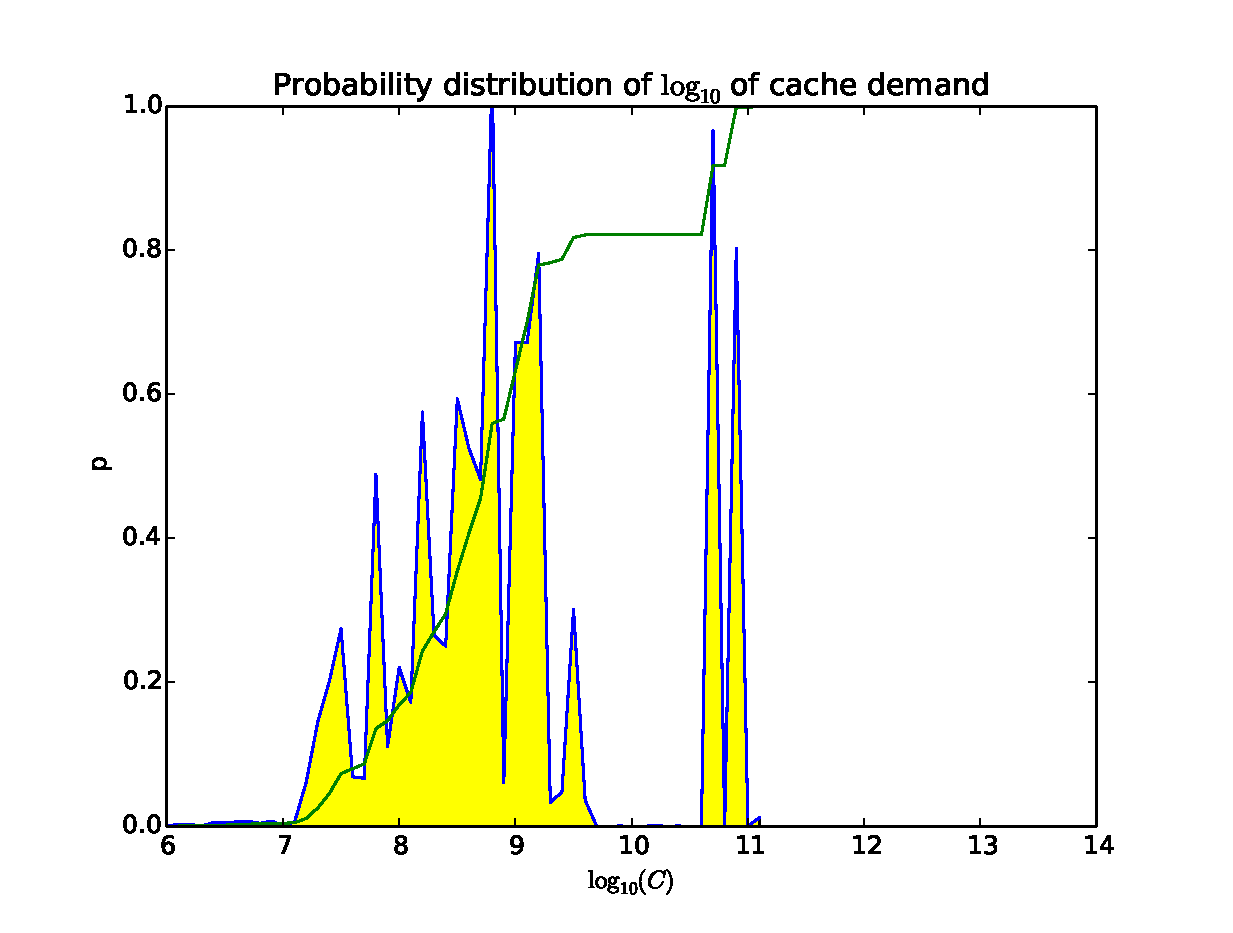
\includegraphics[width=65mm]{ocfa/step2/stripped1_virtcachesize.eps}
}
\subfloat[second]{
  \includegraphics[width=65mm]{ocfa/step2/stripped2_virtcachesize.eps}
}
\hspace{0mm}
\subfloat[third]{
  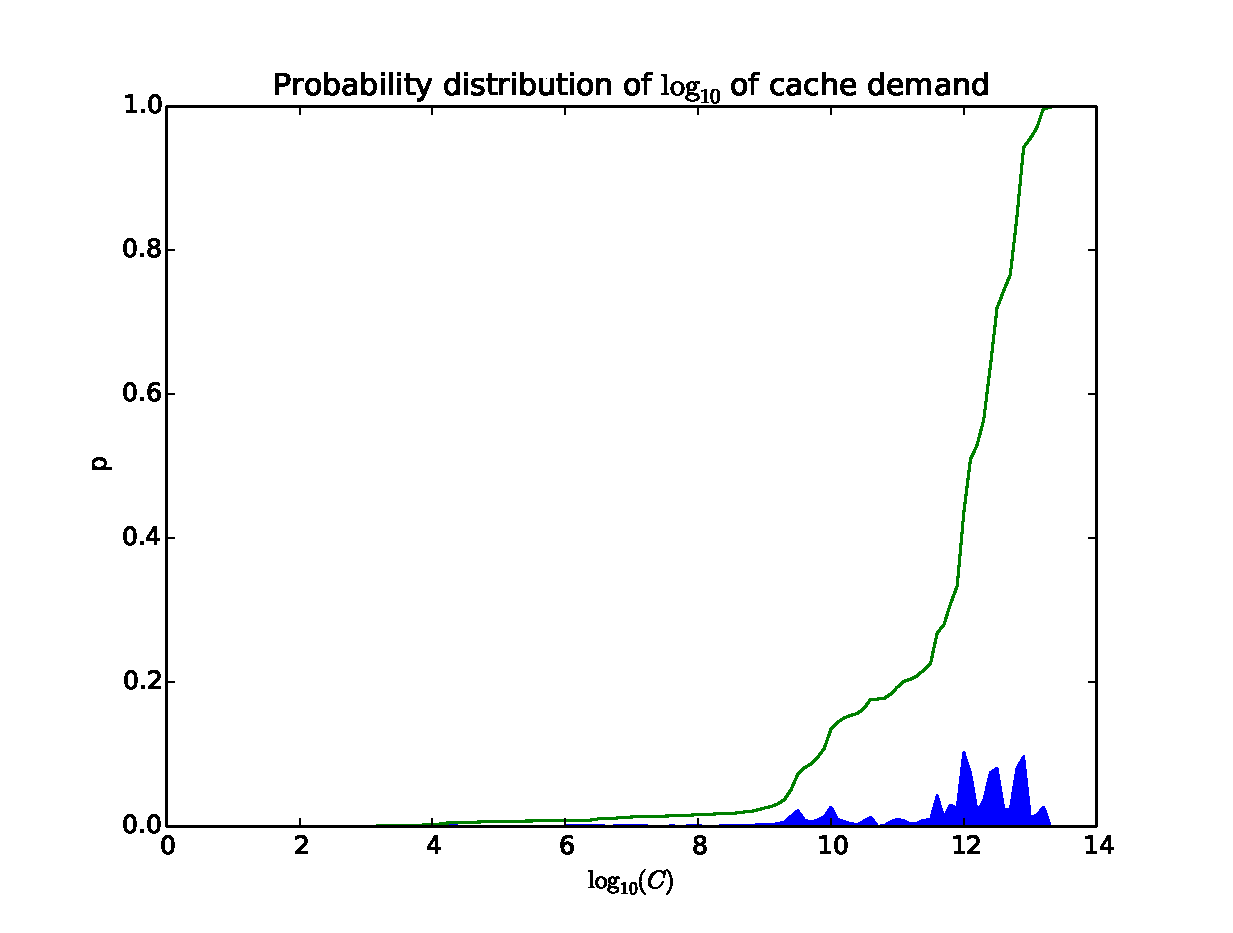
\includegraphics[width=65mm]{ocfa/step2/stripped3_virtcachesize.eps}
}
\subfloat[forth]{
  \includegraphics[width=65mm]{ocfa/step2/stripped4_virtcachesize.eps}
}
\caption{Virtual cache size propability density}
\end{figure}

\section{Inter-job timing}
FIXME, we need text here.
\begin{figure}
\centering
\subfloat[case 1]{
  \includegraphics[width=70mm]{ocfa/step3/stripped1_prevnext_by_count.eps}
}
\subfloat[case 2]{
  \includegraphics[width=70mm]{ocfa/step3/stripped2_prevnext_by_count.eps}
}
\hspace{0mm}
\subfloat[case 3]{
  \includegraphics[width=70mm]{ocfa/step3/stripped3_prevnext_by_count.eps}
}
\subfloat[case 4]{
  \includegraphics[width=70mm]{ocfa/step3/stripped4_prevnext_by_count.eps}
}
\caption{Inter-job time probability density}
\end{figure}
\section{Inter-job timing by content size}
FIXME, we need text here.
\begin{figure}
\centering
\subfloat[case 1]{
  \includegraphics[width=70mm]{ocfa/step3/stripped1_prevnext_by_size.eps}
}
\subfloat[case 2]{
  \includegraphics[width=70mm]{ocfa/step3/stripped2_prevnext_by_size.eps}
}
\hspace{0mm}
\subfloat[case 3]{
  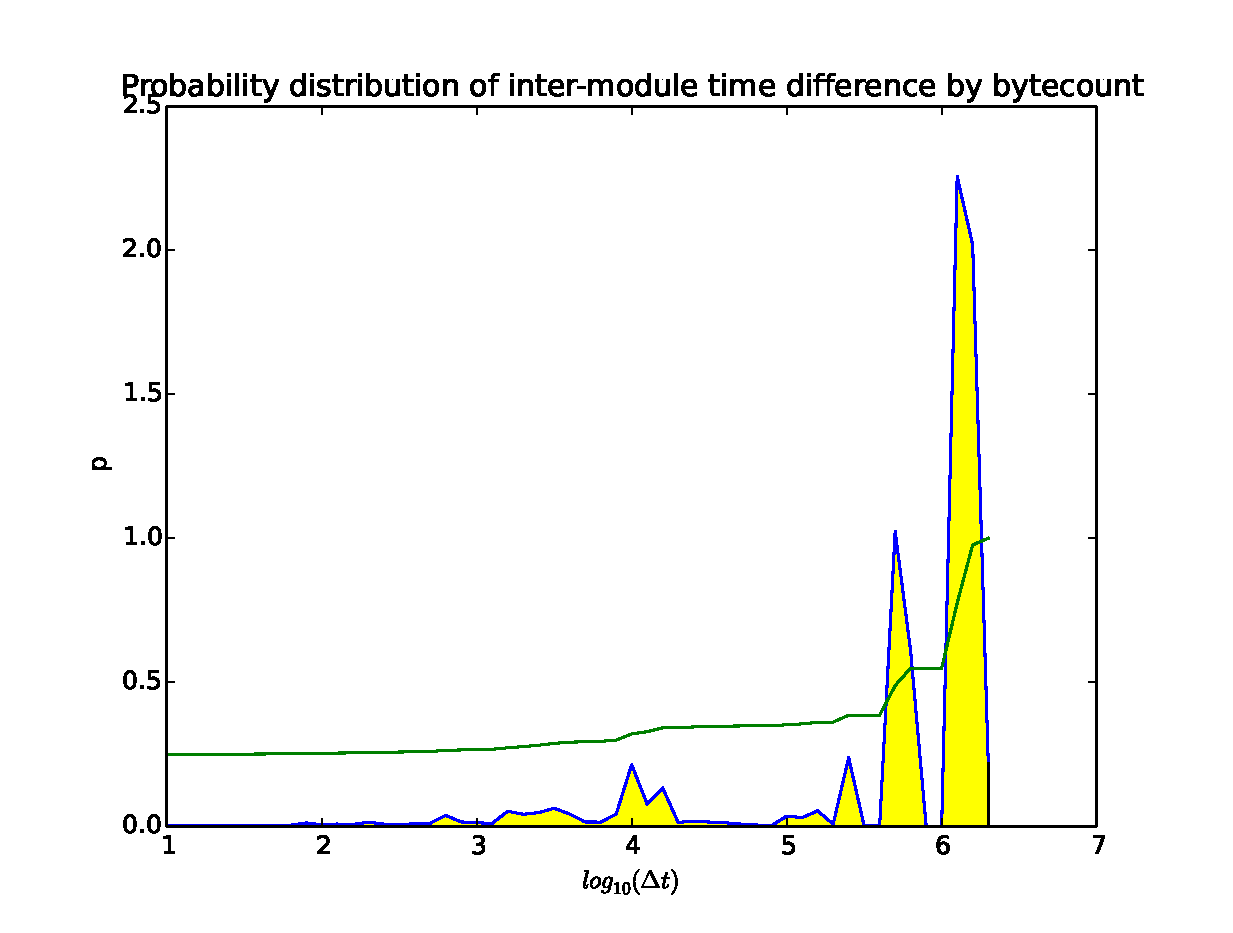
\includegraphics[width=70mm]{ocfa/step3/stripped3_prevnext_by_size.eps}
}
\subfloat[case 4]{
  \includegraphics[width=70mm]{ocfa/step3/stripped4_prevnext_by_size.eps}
}
\caption{Inter-job time probability density by volume}
\end{figure}
\section{First-last timing}
FIXME, we need text here.
\begin{figure}
\centering
\subfloat[case 1]{
  \includegraphics[width=70mm]{ocfa/step3/stripped1_startstop_by_count.eps}
}
\subfloat[case 2]{
  \includegraphics[width=70mm]{ocfa/step3/stripped2_startstop_by_count.eps}
}
\hspace{0mm}
\subfloat[case 3]{
  \includegraphics[width=70mm]{ocfa/step3/stripped3_startstop_by_count.eps}
}
\subfloat[case 4]{
  \includegraphics[width=70mm]{ocfa/step3/stripped4_startstop_by_count.eps}
}
\caption{First-last time probability density}
\end{figure}
\section{First-last timing by content size}
FIXME, we need text here.
\begin{figure}
\centering
\subfloat[case 1]{
  \includegraphics[width=70mm]{ocfa/step3/stripped1_startstop_by_size.eps}
}
\subfloat[case 2]{
  \includegraphics[width=70mm]{ocfa/step3/stripped2_startstop_by_size.eps}
}
\hspace{0mm}
\subfloat[case 3]{
  \includegraphics[width=70mm]{ocfa/step3/stripped3_startstop_by_size.eps}
}
\subfloat[case 4]{
  \includegraphics[width=70mm]{ocfa/step3/stripped4_startstop_by_size.eps}
}
\caption{Firtst-last time probability density by volume}
\end{figure}

\section{Inflow and outflow for our ficticious cache}
FIXME, we need text here.
\begin{figure}
\centering
\subfloat[first]{
  \includegraphics[width=65mm]{ocfa/step4/stripped1_inflow.eps}
}
\subfloat[second]{
  \includegraphics[width=65mm]{ocfa/step4/stripped2_inflow.eps}
}
\hspace{0mm}
\subfloat[third]{
  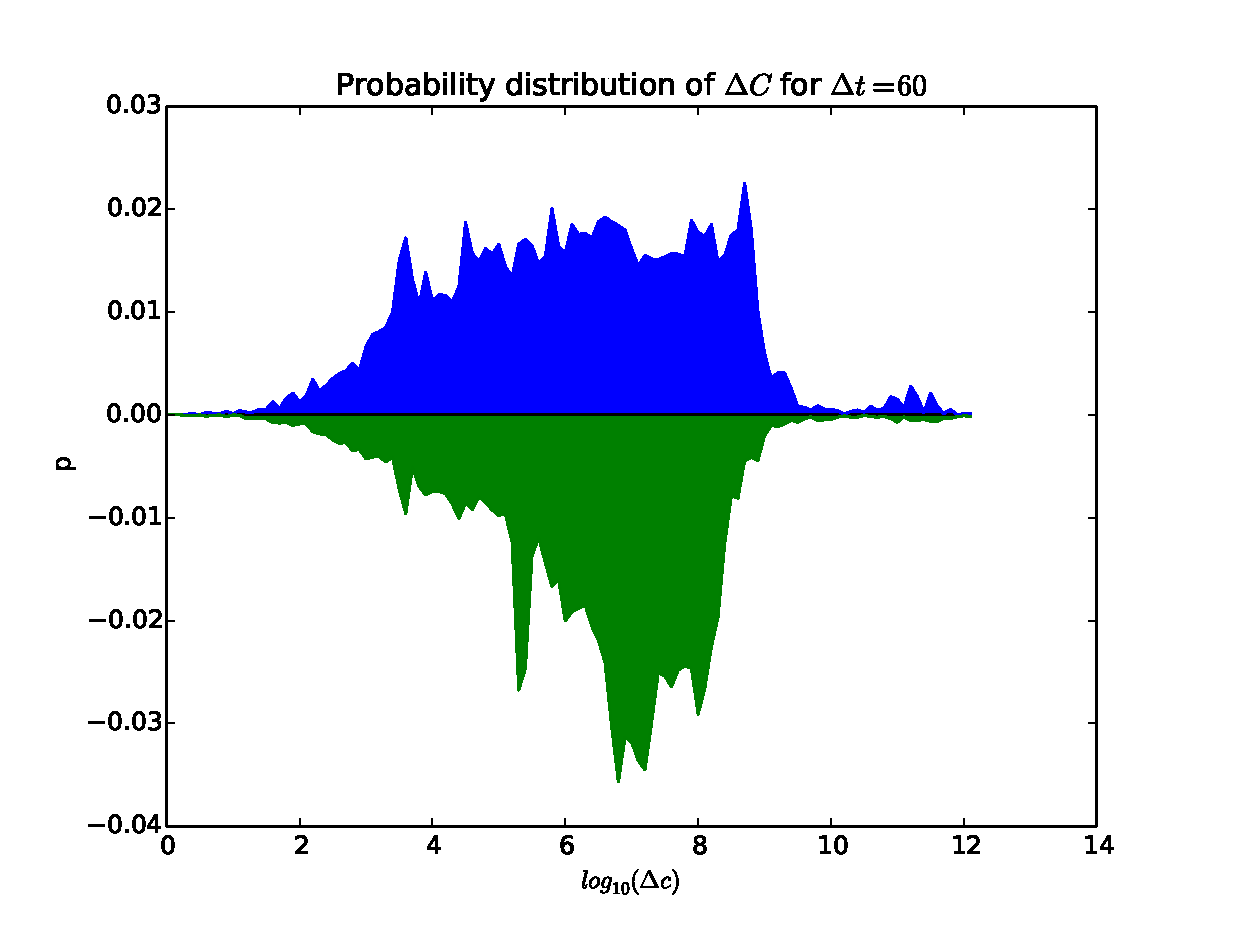
\includegraphics[width=65mm]{ocfa/step4/stripped3_inflow.eps}
}
\subfloat[forth]{
  \includegraphics[width=65mm]{ocfa/step4/stripped4_inflow.eps}
}
\caption{In/out flow probability density}
\end{figure}

\section{Inter-module flows}
FIXME: we need text here.
\begin{figure}
  \centering
  \includegraphics[width=130mm]{ocfa/step5/stripped1_modules.eps}
  \caption{Case 1 inter-module flows}
\end{figure}
\begin{figure}
  \centering
  \includegraphics[width=130mm]{ocfa/step5/stripped2_modules.eps}
  \caption{Case 2 inter-module flows}
\end{figure}
\begin{figure}
  \centering
  \includegraphics[width=130mm]{ocfa/step5/stripped3_modules.eps}
  \caption{Case 3 inter-module flows}
\end{figure}
\begin{figure}
  \centering
  \includegraphics[width=130mm]{ocfa/step5/stripped4_modules.eps}
  \caption{Case 4 inter-module flows}
\end{figure}
\begin{figure}
\centering
\subfloat[case 1]{
  \includegraphics[width=70mm]{ocfa/step5/stripped1_modtypes.eps}
}
\subfloat[case 2]{
  \includegraphics[width=70mm]{ocfa/step5/stripped2_modtypes.eps}
}
\hspace{0mm}
\subfloat[case 3]{
  \includegraphics[width=70mm]{ocfa/step5/stripped3_modtypes.eps}
}
\subfloat[case 4]{
  \includegraphics[width=70mm]{ocfa/step5/stripped4_modtypes.eps}
}
\caption{Rough data flow}
\end{figure}

\section{Conclusions of the OCFA timing analysis}
In this section we look at the information gathered from analyzing the OCFA timing info from four investigations and try to draw well foundedconclusions from this data by combining it with knowledge about the OCFA architecture.
\subsection{Effectiveness of OCFA throughput measures}
As we have seen in the event based graphs looking at the probability density of per data entity timing, the priority queuing would seem to be effective, and would probably be quite effective if all data entities were similarly sized. Looking though at the data volume compensated probability density graphs, we see that the effectiveness of priority queuing becomes questionable at best. We don't have sufficient proof to state that the measure may be anti productive from a cache hit rate point of view, but its something that at this point in time seems like a viable hypothesis. A hypothesis though that we must leave untested as there is no comparative material available to test it. It is safe to say though that from a cache-hit efficiency point of view, the priority queuing mechanism proves to be at best insufficient.
\subsection{The effects of meta-data messaging inefficiency and centralized router}
One of the known performance bottlenecks of OCFA is the implementation of the meta-data access. Conceptually an evidence entity is forwarded between modules through the messaging system. Due to monitoring concerns though, an approach was taken where short messages were used instead with an internal reference to a BLOB inside of the Postgres database. The process for processing and forwarding an evidence entity to a module or router is the following:
\begin{itemize}
\item Module receives an incoming message from the Anycast relay.
\item Module extracts the meta-data ID from the message
\item Module retrieves the XML blob containing the evidence trace from Postgres
\item Module validates and parses the XML into a DOM tree
\item Module extracts the data ID from the XML
\item Module retrieves the evidence data filesystem path from Postgres
\item \emph{Process the data}
\item Module adds additional meta-data to the DOM tree.
\item Module serializes the DOM tree to a new version of the XML trace
\item Module updates the XML BLOB in the Postgres database
\item Module sends a return message to the Anycast asking to forward it to the router.
\item Anycast marks the old message as processed and places the new message in the router queue.
\item When router queue reaches message, Anycast sends message to the router
\item Router receives an incoming message from the Anycast relay.
\item Router extracts the meta-data ID from the message
\item Router retrieves the XML blob containing the evidence trace from Postgres
\item Router validates and parses the XML into a DOM tree
\item Router traverses the meta-data and determines the next module to process the evidence entity
\item Router adds additional meta-data to the DOM tree.
\item Router serializes the DOM tree to a new version of the XML trace
\item Router updates the XML BLOB in the Postgres database
\item Router sends a return message to the Anycast asking to forward it to the specific next module.
\item Anycast marks old message as processed and places the new message in the router queue.
\item When router queue reaches message, Anycast sends message to the next module
\item When module queue reaches message, Anycast sends message to the next module
\end{itemize}
It's easy to see that there is quite some overhead in messaging and routing.
There are a number of known bottlenecks in this process that would be suitable for addressing the speed of the OCFA framework. While these bottlenecks aren't part of the subject of this thesis, it is important to note them for a complete picture of messaging based bottlenecks:
\begin{itemize}
\item With an ever growing relational database, the retrieving and updating of XML in the database becomes a major bottleneck. Using the XML directly in the messaging system would have much better scaling properties. This would come at the expense of monitoring possibilities and there will be no intermediate results until the evidence would be fully processed. 
\item As with the previous item, with an ever growing relational database, the retrieving of the evidence data filesystem path from the database becomes a major bottleneck. Storing the evidence data path directly in the message itself should have significantly better scalability. Again however this would come at the expense of monitoring possibilities.
\item The use of XML, XML-schema and related technology was very much current when OCFA was designed. In retrospect though, XML is a highly expensive serialization technique and other serialization possibilities like JSON or FlatBuffers
would likely have been significantly less overhead. Further, a custom container format that could simply append a job record rather than serialize the whole trace on each communication step would make re-serialization significantly more efficient.
\item The use of a separate router process makes that much of the overhead is repeated twice. Moving the router functionality into the messaging library and thus into the module processes should de-duplicate this overhead and make for a major overhead reduction. 
\end{itemize}
So to summarize, there is quite some room for improvement in the efficiency of the cross module timing. We can assume that any future OCFA successor that aims to use a similar message based concurrency model will implement such improvements. The subject of this thesis though is concerned not with these particular efficiency issues but with issues related to disk-cache hit rates. So how would faster inter-module communication affect the timing we have seen in our evaluation? Some considerations:
\begin{itemize}
\item More efficient inter-module messaging, especially with respect to the database bottlenecks, could significantly speed up the frequency at which the main kickstart and carving functionality, and other evidence entity producers could increase the amount of \emph{active} data in the system. 
\item The per-module overhead is most dominant in fast modules and in the full processing of smaller files. It stands to reason that the observed inefficiency of priorities for larger data entities would thus further deteriorate.
\item As has been observed in the past when running additional routers on additional CPU's or servers, the presence of the routing bottleneck serves as a major enabler for the priorities system. Given that the priorities work on a per module basis, without a router bottleneck the priority system only works with other bottleneck modules. The router bottleneck works as a distribution point for the priority queuing. Combined with the previous point this could very well mean that an increase in performance using the measures above would fully deprecate the usefulness of such per message queue based priorities. 
\end{itemize}
\subsection{Conclusions and lessons learned}
From the analysis of the timing information from four real life OCFA runs, and our knowledge of the OCFA system we can draw some conclusions regarding the inability of the OCFA design to effectively minimize the amount of disk-cache misses and with respect to what may be improved in the design of a new OCFA-like system that could improve both the disk-cache efficiency and the overall throughput of the system.
\begin{itemize}
\item The un-throttled input of new data into the system creates an imbalance between inflow and outflow that leads to much higher amount's of \emph{active} data than can be accounted for by disk cache, inevitably leading to massive amounts of disk cache misses. A form of throttling for new data submission is a necessity for effectively addressing disk cache efficiency.
\item The percentage of data that is discarded after a file-type check is significant when compared to the percentage of data that is discarded after a hash value check. It would seem logical to design a new system in such a way that file-type checking happens before the file is actually read by the framework, as to remove unneeded overhead from reading the file data, either to copy it out or to determine the file hash. This seems one argument in favor of opportunistic hashing. 
\item When looking at the chain of modules that processes particular data, it is not uncommon for the first full read to be the result of the on-creation hashing, while the second and often last full read happens in the last module before the (in OCFA) meta-data-only Data Store Module. This means that if hashing could be delayed to a later module, that while the entity processing time may stay approximately the same, the disk-cache hit probability could improve resulting from the reduced first full-read last full-read timing. 
\item The percentage of data that constitutes large entities without in anyway meaningful hash value (such as whole partitions or unallocated space cluster collections) makes up a majority of all data processed. Traversing such large data chunks for the sole purpose of calculating a set of hashes, as is done in the OCFA architecture is wasteful. This seems a second argument in favor of opportunistic hashing.
\item The percentage of larger data that is processed that is a chunk of other data being processed is significant. This implies that the disk cache size requirements could be reduced by making extensive use of annotation based addressing such as in CarvFS.
\end{itemize}
So basically, from a disk-cache efficiency viewpoint, we are proposing three distinct yet interdependent measures:
\begin{itemize}
\item \emph{Opportunistic hashing}: Calculate hashes opportunistically when an entity as a whole is either being written or read or explicitly when the hashes are needed for further processing.
\item \emph{Annotation based data access}: Use a CarvFS alike system for accessing data as chunks within a bigger whole.
\item \emph{New-data input throttling}: Keep track of \emph{active} data in the system and throttle input accordingly.
\end{itemize}
While not the core subject of this dissertation, the following improvements to an OCFA like  forensic framework design should be beneficial given that the above disk-cache related issues are solved first:
\begin{itemize}
\item Integration of router functionality into the messaging library.
\item Integration of file-type module (libmagic) functionality into the messaging/router library.
\item Full-meta-data messaging separate from central database storage. No intermediate result storage in database.
\item Use of more efficient serialization technology instead of XML.
\end{itemize}


\chapter{Scripts created for OCFA timing analysis}
\noindent 
\renewcommand{\bibname}{Scripts}
\begin{thebibliography}{1}
\bibitem{strip2} strip2.py, {\em Script for extracting timing information from an OCFA  Postgres database dump}  \url{https://github.com/pibara/mattock-dissertation/blob/master/ocfa/step1/strip2.py}
\bibitem{eventdump} eventdump.py, {\em Script for extracting first occurrence/last occurrence event from an OCFA time-info dump} \url{https://github.com/pibara/mattock-dissertation/blob/master/ocfa/step2/eventdump.py}
\bibitem{virtcachesize} virtcachesize.py {\em Script for generating probability density graph of fictitious cache size}  \url{https://github.com/pibara/mattock-dissertation/blob/master/ocfa/step2/virtcachesize.py}
\bibitem{intervals} intervals.py {\em Script for generating wide range of timing interval PD graphs}  \url{https://github.com/pibara/mattock-dissertation/blob/master/ocfa/step3/intervals.py}
\bibitem{inflow} inflow.py {\em Script for generating a set of inflow/outflow PD function graphs}  \url{https://github.com/pibara/mattock-dissertation/blob/master/ocfa/step4/inflow.py}
\bibitem{flow2dot} flow2dot.py {\em Script for generating a cross-module data-flow diagram} \url{https://github.com/pibara/mattock-dissertation/blob/master/ocfa/step5/flow2dot.py}
\bibitem{genflow2dot} genflow2dot.py {\em Script for generating a consolidated version of the cross-module data-flow diagram}  \url{https://github.com/pibara/mattock-dissertation/blob/master/ocfa/step5/genflow2dot.py}
\end{thebibliography}

\chapter{Page-cache in the Linux operating-system}
In this appendix we examine the core properties of the Linux page-cache and the possibilities for interacting with the page-cache and related memory layout parameters in a way that could limit the disk-cache miss rate of a multi-process system running on this OS. First we will look at the main memory usage strategy used by Linux and at the way that page-cache competes for RAM with other RAM consuming Linux subsystems. We will look at information we can extract from the virtual /proc filesystem and at POSIX APIs that provide a way to interact with the way the page-cache works. We than move on to project this knowledge to our ficticious computer-forensic framework and discuss what measures can be taken to effectively interact with the Linux system in order to limit page-cache misses on a Linux system that is hosting such a framework. We close this appendix by reasoning about possible strategies that could be used by a computer-forensic framework in an attempt to optimize disk-cache hit percentages while at the same time not introducing other sources of stagnating troughput to the resulting setup.
\section{Allocation and use of page-cache}
RAM in a computer is a shared resource. It is a scarce resource that is managed by the operating system. The OS kernel itself runs in RAM as do the user processes. Both kernel/process code, heap and stack take up pieces of RAM and on a bussy system some RAM pages may end up getting swapped out of RAM to an on-disk swap facility. Not all RAM is kept available to kernel and processes. Part of RAM is allocated to hold a copy of on-disk data and to act as a cache for file data that the Linux kernel assumes is likely to be read again in the forseeable future, allowing for more efficient use of the relatively slow reading from hard disk media. An other part is allocated to temporary hold data pages that should eventualy end up on disk and arn't synced to disk yet as to improve the overall system performance related to issues with frequent short writes. The Linux kernel needs to balance the desire to avoid wasting disk-IO on swapping out process memory with the desire to not waste disk-IO on data that could have been cached. Its like there is a rubber band between the process oriented RAM usage and the file-IO orented RAM usage. As such, memory available to page-cache is not static. It depends on the process behaviour of the different processes on the system. Our main interest in RAM for the purpose of this research is an interest in the part of the RAM used for the read-part of the page cache. While there is a lot to say about the use and tuning of write oriented caches, this falls outside of the scope of this paper and thuss shall not be discussed here. 
\section{/proc/meminfo}
In the /proc filesystem, the pseudo file /proc/meminfo can be used to access kernel information about the size and use of the system RAM. Some potentialy interesting variables that can be retreived from this pseudo file are:
\begin{itemize}
\item \emph{Cached} : In-memory cache for files read from dish (the pagecache).
\item \emph{MemFree} : The total of memory that is free to be used for anything.
\item \emph{Active} : Recently used memory that idealy isn't reclaimed.
\item \emph{MemTotal} : The total usable system RAM.
\item \emph{SwapTotal} : Total amount of swap space available.
\item \emph{SwapFree} : The currently unused portion of the swap space.
\end{itemize}
The information from this pseudo file can be used to initialize or later tune our efforts at throtling data input into our system. 
\subsection{Starting off with a clean slate}
If we want to repeatedly run tests with the page-cache behaviour of the system, it will be important that we can reinitialize our page-cache so that a first test does not mess with a second or third test. So how do we reinitialize the page cache so we can start our test with a clean slate? There are two things we need to do.  First make sure all page cache \emph{can} be initialized cleanly by invoking \emph{sync} as root. After that we run the following command (as root):
\begin{itemize}
\item \emph{echo 3 > /proc/sys/vm/drop\_caches}
\end{itemize}
This command will write the number \emph{3} to the pseudo file /proc/sys/vm/drop\_caches. Doing so will prompt the kernel to free the cache and slab objects. 
\section{API interaction with the page-cache part of the Linux kernel}

\section{Interaction between a computer-forensic framework and the Linux kernel}
\section{Possible strategies}
\section{Conclusions}


\chapter{MattockFS: A CarvFS successor.}
In this appendix we describe the functionality and design of a new user-space file-system. MattockFS is meant to be a successor to the user space file-system named CarvFS that was released by the Dutch National Police in 2010 to act as an annotation based pseudo file-system aimed at facilitating zero-storage carving to the OCFA forensic framework. While CarvFS was retrofitted to work with OCFA, we aim to create a new user-space file-systemed modeled partially after CarvFS that should act as the potential foundation of new message passing oriented forensic framework. We envission that MattockFS, together with a serialization library and message bus technology could form the foundation for a yet ficticious future \emph{Mattock} forensic framework, loosely modeled after the OCFA forensic framework. The aim is to implement as much as is logical and sensible of the main aspects of disk-cache optimization techniques into this user space file-system. This should include facilities for querying throttling relevant information, facilities for keeping track of \emph{active} CarvPaths, facilities for marking expected read-access patterns for a given CarvPath and for marking a CarvPath as no longer needed. Also it shall include facilities for opportunistic hashing. Finaly, while in OCFA, the concept of a growing archive was implemented by allowing a data-generating module access to the raw data-file underlying the file-system, in MattockFS we shall opt to implement this trough a file-system layer.
\section{FUSE: File-system in userspace}
\section{MattockFS functionality}
\subsection{Adding data to the archives}
\subsection{Annotation based data access}
\subsection{Framework usage vs interactive usage}
\subsection{Page usage controll, monitoring \& release}
\subsection{Throtling controll}
\subsection{Opportunistic hashing}
\subsection{Distributed access concerns}
\section{Sub-functionality in shared libraries}
\subsection{LibCarvPath++: A C++ CarvPath annotation library}
\subsection{LibCarvStack++: A C++ CarvStack library}
\section{Required file-system interfaces}
\section{An extended attribute based control interface}
\section{Convenience API's}
\subsection{LibMattockFS++ \& PyMattockFS: Extended-attribute interface wrappers for C++ and Python}
\subsection{PyCarvPath: A Python port of LibCarvPath++}

\end{appendices}

\end{document}
